\section{Node Model}\label{sec:impl-node}

Bitcoin is a decentralized network of nodes. Thus, the node is the core
component of \iblock{}.

Nodes in \iblock{} are compound modules composed of various \emph{applications}
--- simple modules that handle specific tasks. All applications inherit from
the \code{AppBase} class, which provides foundational features, making it
easier to add new functionalities.

Nodes in \iblock{} are highly modular: users can tailor a node's capabilities
by selecting different applications, allowing each node to exhibit unique
functionality.

Since a Bitcoin node maintains its own state defined by the \emph{blockchain}
and \emph{mempool}, every \iblock{} node includes two essential applications:
the \code{BlockchainManager} for blockchain management and the
\code{MempoolManager} for mempool management. Additional applications can be
added to customize node behavior using NED language.

Each \iblock{} node maintains \emph{its own perspective} of the blockchain and mempool,
just like nodes in a real Bitcoin network. This means one node's blockchain or
mempool may differ from another's, as nodes may have different blocks or
transactions at any point in time.

\figref{fig:node-internals} shows a miner node configured with transaction
generation capabilities. Internal communication between applications and with
global modules uses Direct Method Calls (DMCs), while node-to-node
communication relies on messages. The figure illustrates key interactions
between applications within a node.

\begin{figure}[tbhp]
	\centering
	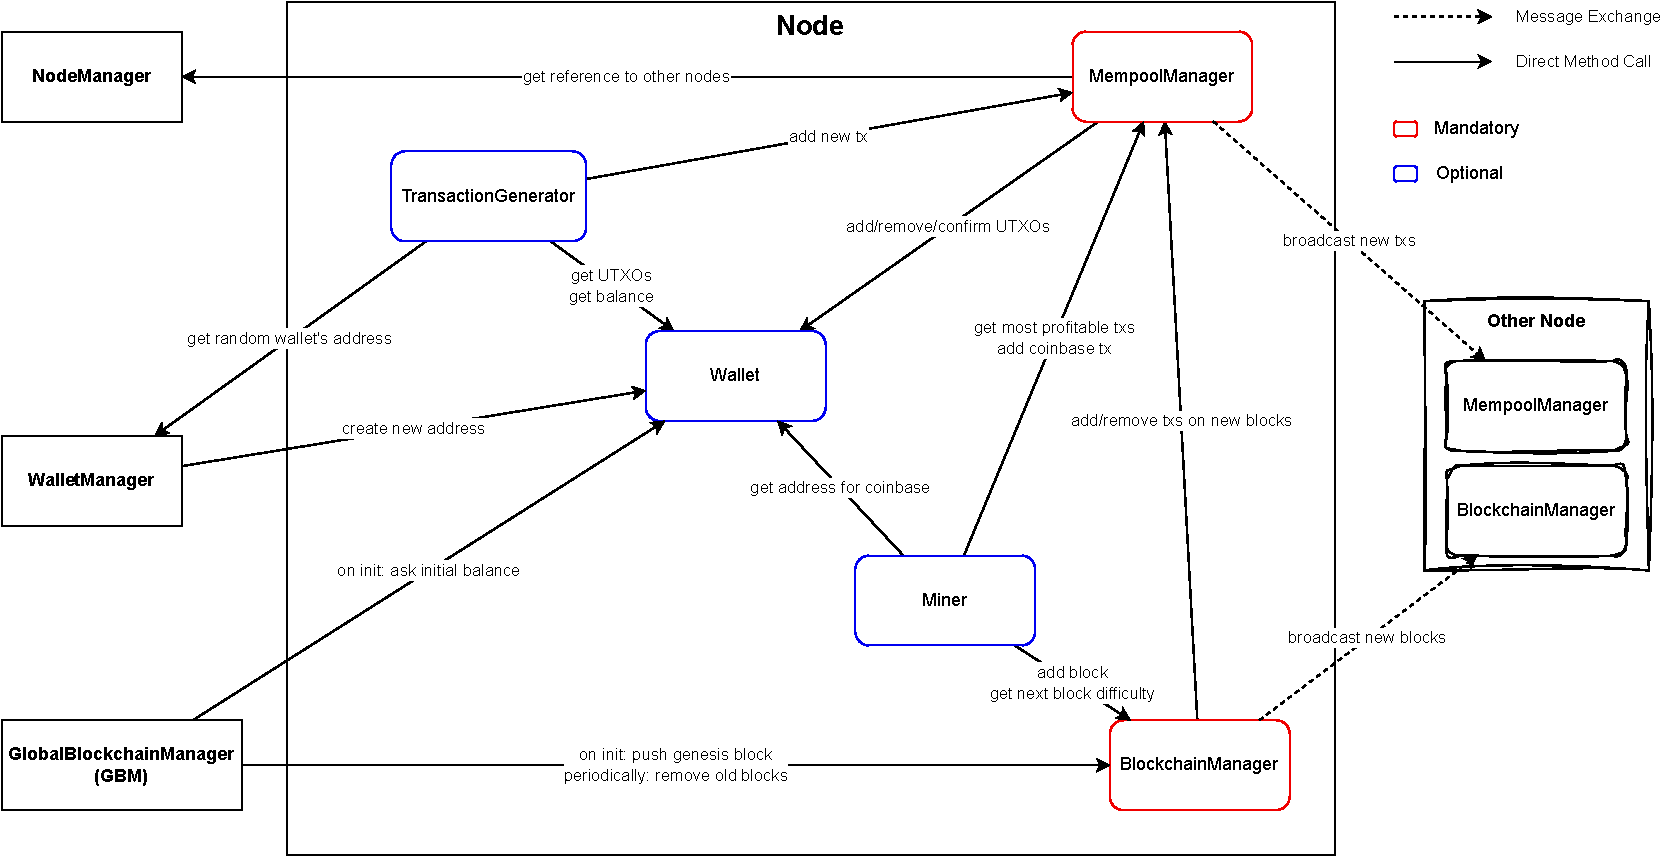
\includegraphics[width=\textwidth]{node-internals}
	\caption{Structure of a node, showing internal applications and main
	communication flows.}\label{fig:node-internals}
\end{figure}

\subsection{Applications}\label{subsec:applications}

The applications that make up a node allow for behavior customization by simply
editing NED and configuration files, eliminating the need to alter C++ source
code. \figref{fig:app-inheritance} shows the inheritance structure for
applications. Using the \code{IApp} interface, users can switch the
implementation of specific applications through configuration alone. For
instance, to replace the standard \code{BlockchainManager} with a
\code{SelfishBCManager} (see \secref{sec:selfish-poc}), a single line in the
configuration file suffices:

\footnotesize
\begin{verbatim}
Network.node[0].blockchainManager.typename = "iblock.bitcoin.apps.SelfishBCManager"
\end{verbatim}
\normalsize

\begin{figure}[tbh]
	\centering
	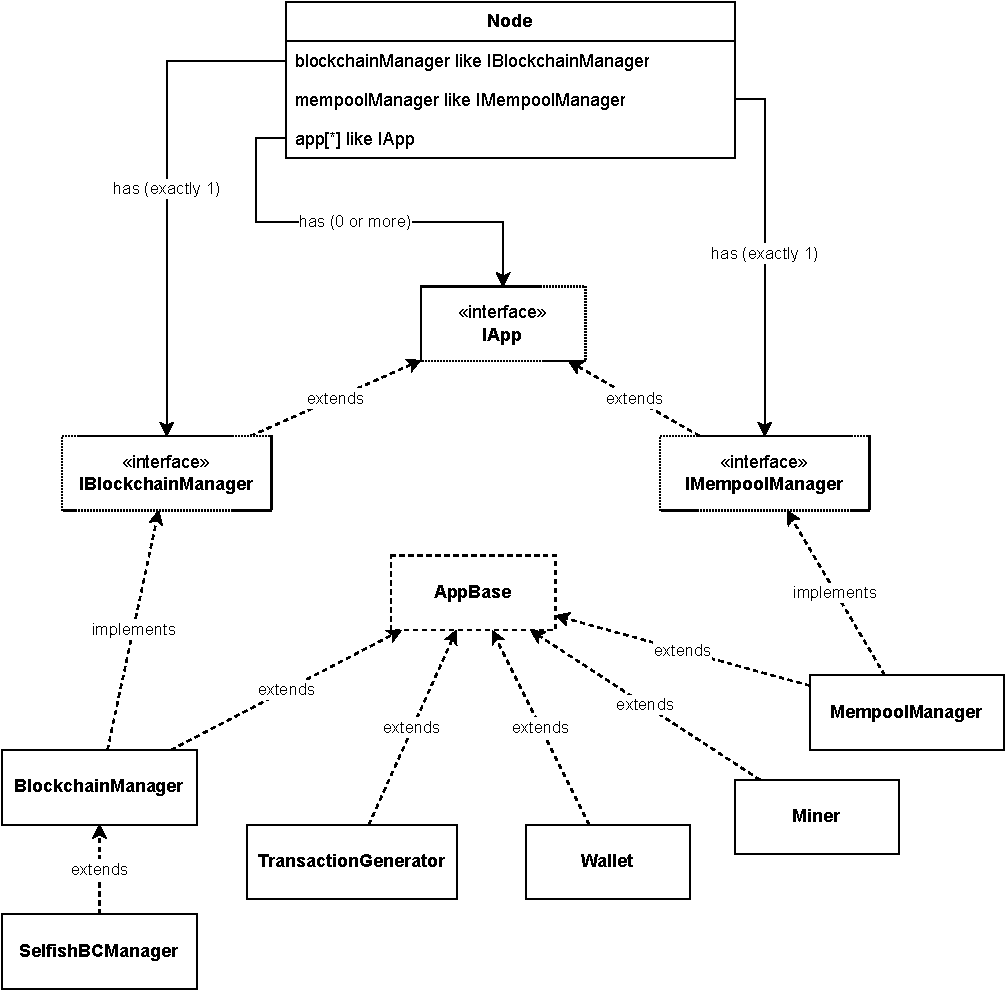
\includegraphics[width=0.8\textwidth]{apps-inheritance}
	\caption{Inheritance tree of applications.}\label{fig:app-inheritance}
\end{figure}

A node may contain several applications: for example, a miner node needs a
\code{Miner} application to mine blocks and a \code{Wallet} application to
receive mining rewards. Nodes generating transactions require a \code{Wallet}
to store coins and a \code{TransactionGenerator} to create transactions.

When a node receives an external message via direct messaging, \code{AppBase}
first processes the message before calling the \code{handleOtherMessage} method
of the application. The reasoning behind this method's name is explained in
\secref{sec:partial-work}.

\figref{fig:app-uml} shows the UML diagram of applications and global modules.
Each application will be described in detail in the following sections.

\begin{figure}[tbhp]
	\centering
	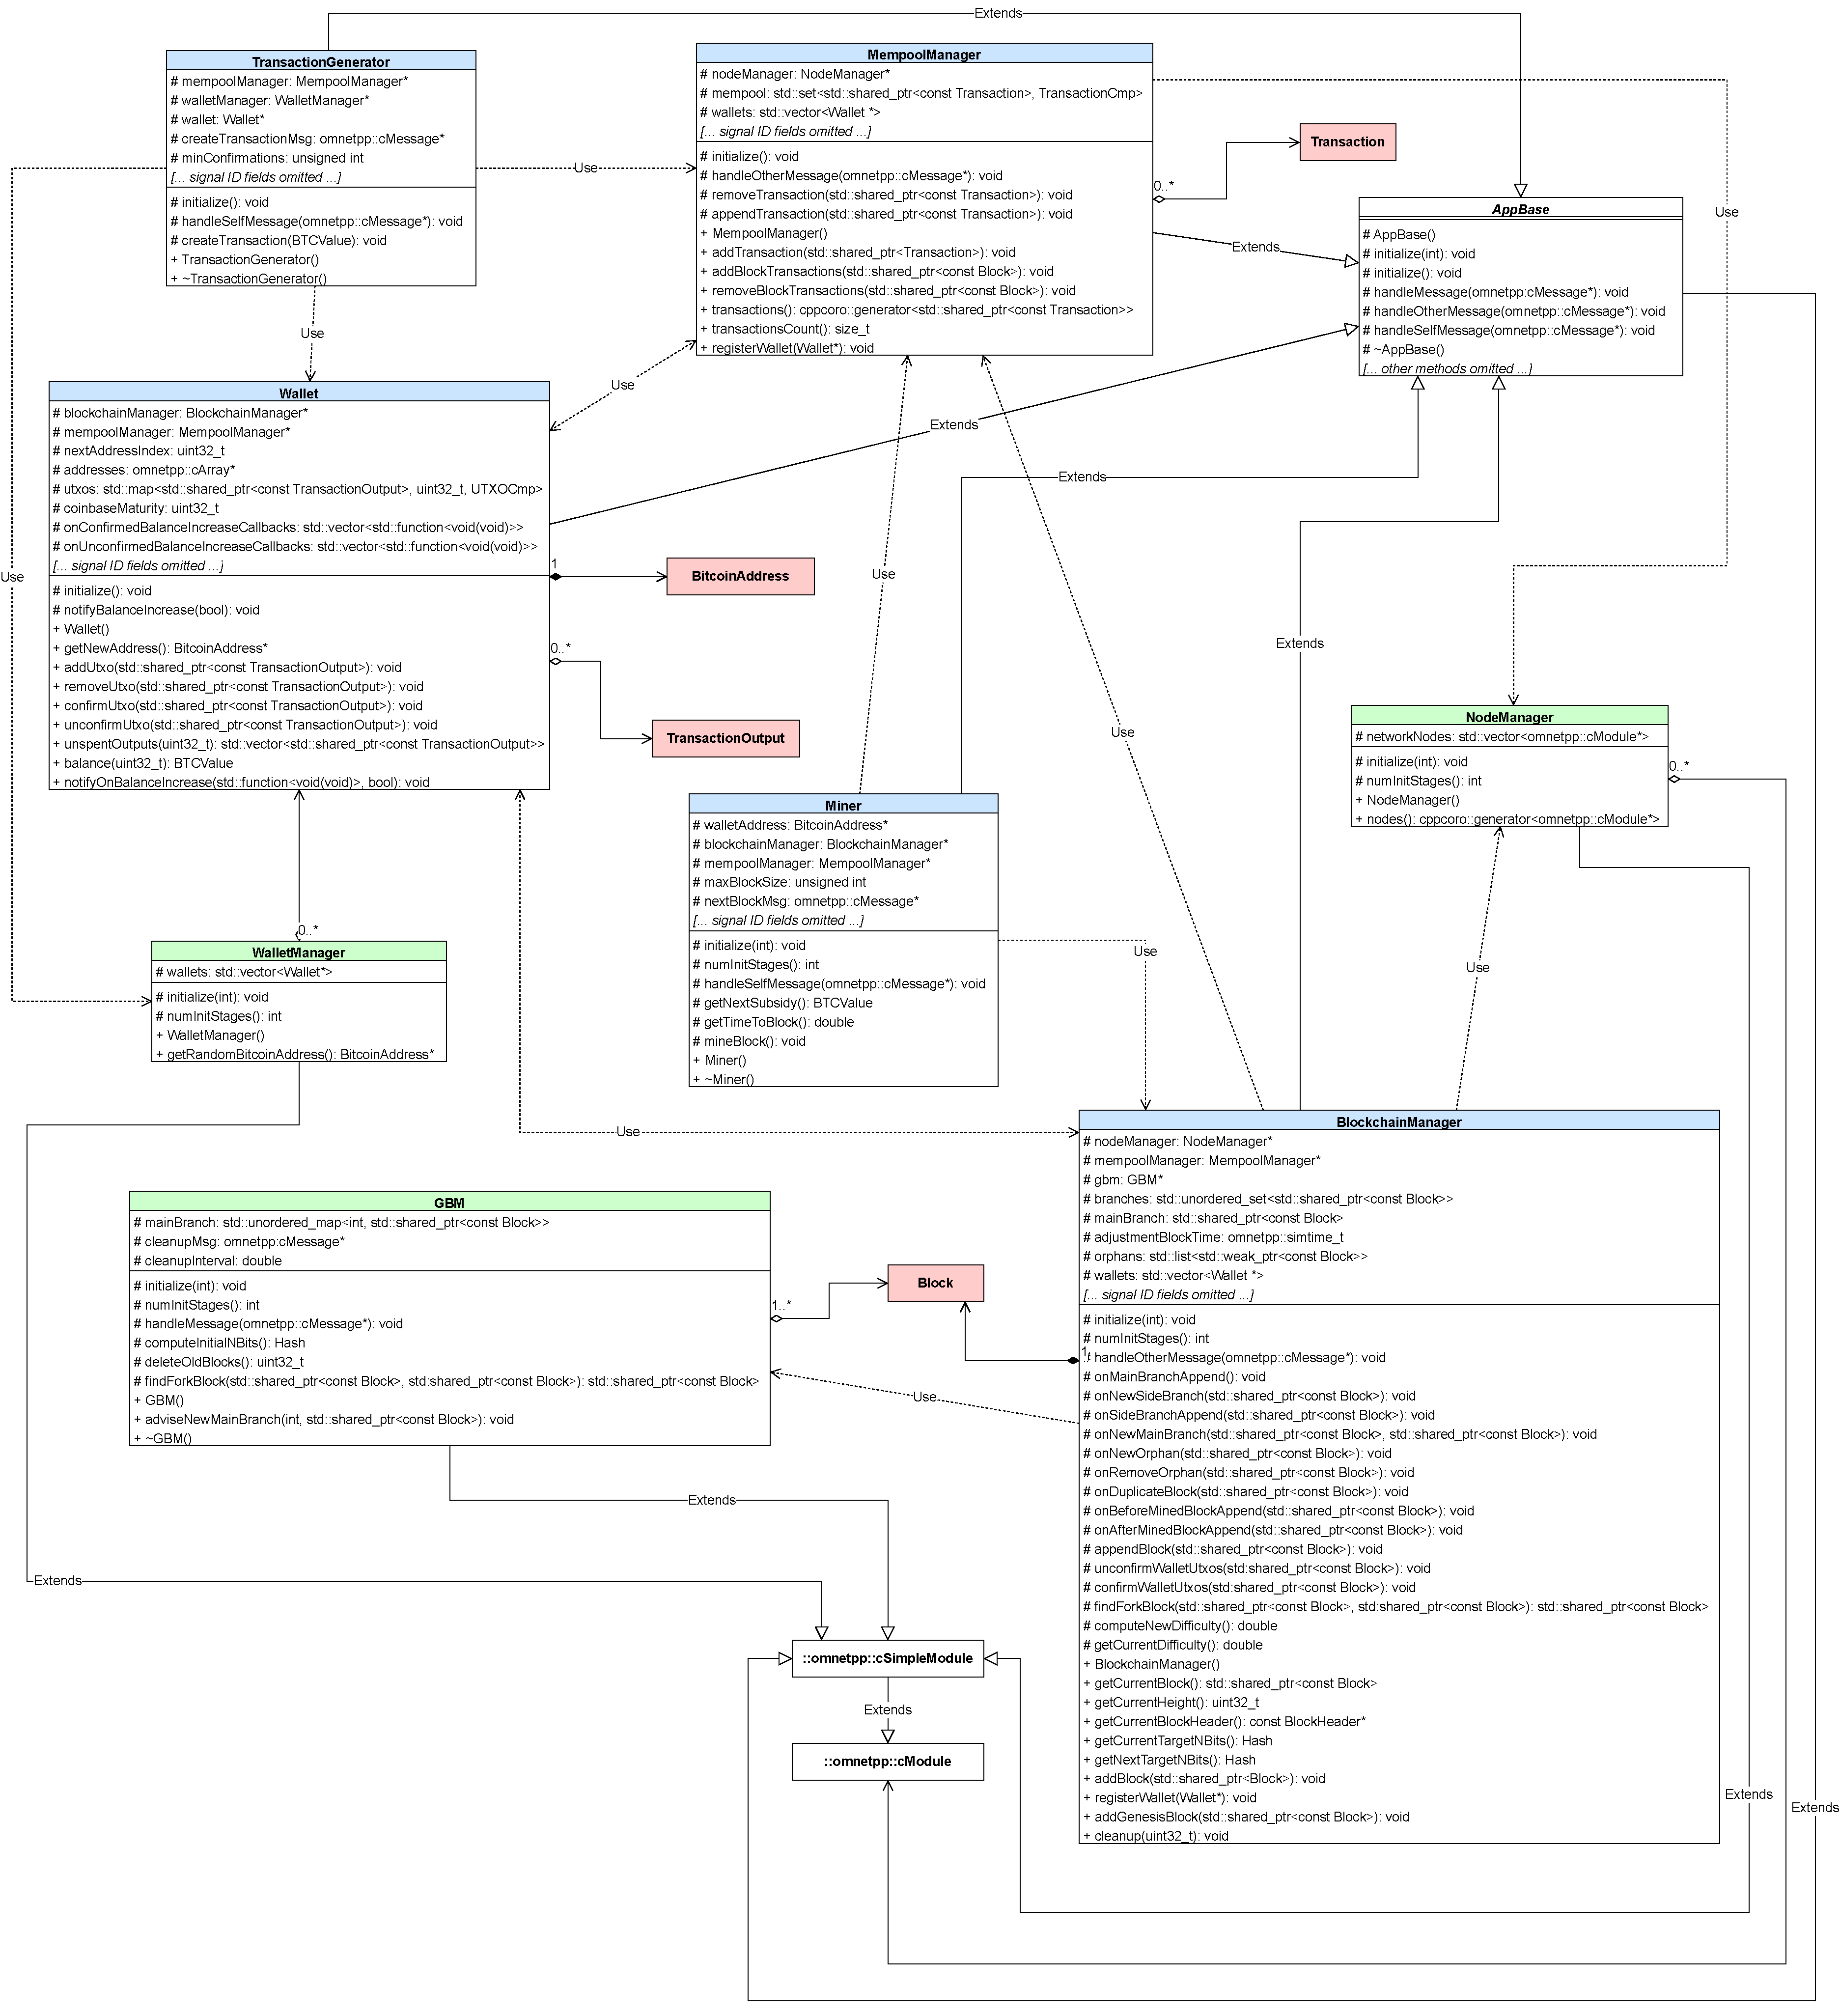
\includegraphics[width=\textwidth]{apps-uml} \caption{Applications and
	global modules UML diagram.}\label{fig:app-uml}
\end{figure}

Both \code{BlockchainManager} and \code{MempoolManager} are required
application for any \iblock{} node to ensure proper blockchain and transaction
pool maintenance.

\subsubsection{BlockchainManager}\label{subsubsec:blockchainmanager}

The \code{BlockchainManager} application manages the blockchain structure for
each node by maintaining pointers to the heads of all blockchain branches, with
the longest branch designated as the main branch. This module is capable of
handling forks, chain reorganizations, and orphan blocks.

When a node mines a new block, it broadcasts it to all other
\code{BlockchainManager} instances in the network. Upon receiving a block,
\code{BlockchainManager}:
\begin{enumerate}
	\item \textbf{Discard duplicate blocks} without further processing;
	\item \textbf{Extends the main branch} if the block builds on it. This
		involves notifying \code{MempoolManager} to remove included
		transactions and updating the \code{Wallet} application to
		adjust the confirmation count for unspent outputs;
	\item \textbf{Handles forks:} If the new block extends a non-main
		branch, it checks if this branch is now the longest. If so, a
		reorganization occurs where the main branch is reverted
		backward to the fork point, updating the mempool and
		unconfirming UTXOs in the wallet. The new branch is then added
		as the main branch, block by block. If the block does not
		create a longer chain, it simply appends it to the branch;
	\item \textbf{Manages orphan blocks:} Orphan blocks, which lack their
		parent block, are stored until the parent arrives. Once
		received, the orphan is added to the blockchain as per the
		steps above.
\end{enumerate}

This process is managed within the \code{appendBlock} method.

\paragraph{Genesis Block and Cleanup}\label{par:genesis-block-and-cleanup}

At the beginning of the simulation, the \code{GBM} (Global Blockchain Manager)
adds the genesis block --- a special block initializing the network's starting
balances --- to each \code{BlockchainManager}.

While the simulation is running, the GBM periodically calls the \code{cleanup}
method of each \code{BlockchainManager} to remove outdated branches, freeing
memory.

\paragraph{Block Propagation and Difficulty
Adjustment}\label{par:blockprop-and-diffadj}

When a new block is mined by the local \code{Miner}, it is the responsibility
of \code{BlockchainManager} to add the block to the blockchain and then forward
the block to the other nodes in the network. This is done by encapsulating the
block in a \code{DirectBlockMsg} message and sending it to all other nodes via
a \code{sendDirect} call. The reference to the other nodes is obtained from the
\code{NodeManager} global module.

Every 2016 blocks, \code{BlockchainManager} recalculates mining difficulty of
the network based on the time needed to mine the last 2016 blocks, as
implemented in the \code{getNextTargetNBits} method. The difficulty computation
is described in \appendixref{appendix:math}.

\paragraph{Parameters}\label{par:bm-parameters}

Table~\ref{tab:blockchain-manager-parameters} lists the configurable parameters
for the \code{BlockchainManager} application.

\begin{table}[tbhp]
	\tiny
	\centering
	\begin{tabularx}{\linewidth}{|r|c|c|X|}
		\toprule
		Name & Type & Default & Description \\
		\midrule
		\code{gbmModule} & string & ``gbm'' & Path to the \code{GBM}
		global module.\\\midrule
		\code{mempoolManagerModule} & string & ``\^{}.mempoolManager''
		& Path to the \code{MempoolManager} application.\\\midrule
		\code{nodeManagerModule} & string & ``nodeManager'' & Path to
		the \code{NodeManager} global module. \\\midrule
		\code{bandwidth} & int (bits/second) & 1 Mbps & Transmission
		duration of blocks is determined by block size and
		bandwidth.\\\midrule
		\code{propagationDelay} & double (time) & exponential(0.42s) &
		Block propagation delay across nodes.\\
		\bottomrule
	\end{tabularx}
	\caption{\code{BlockchainManager}
	parameters.}\label{tab:blockchain-manager-parameters}
\end{table}

\subsubsection{MempoolManager}\label{subsubsec:mempoolmanager}

The \code{MempoolManager} handles the mempool by maintaining an ordered list of
transactions based on fee rate, allowing miners to prioritize transactions for
maximum profitability.

When a node creates a new transaction, it broadcasts the transaction to each
\code{MempoolManager} instance in the network using direct messages. Upon
receiving a transaction, \code{MempoolManager} adds it to the mempool and
notifies the wallet if any new UTXOs are available.

The \code{MempoolManager} class provides methods for adding and removing
transactions from the mempool. When a local application adds a transaction,
\code{MempoolManager} contacts the \code{NodeManager} global module to retrieve
references to all other nodes and then broadcasts the transaction, encapsulated
in a \code{DirectTxMsg} message, to each \code{MempoolManager} in the network.

\paragraph{Parameters}\label{par:mm-parameters}

Table~\ref{tab:mempool-manager-parameters} lists the configurable parameters
for the \code{MempoolManager} application.

\begin{table}[tbhp]
	\tiny
	\centering
	\begin{tabularx}{\linewidth}{|r|c|c|X|}
		\toprule
		Name & Type & Default & Description \\
		\midrule
		\code{nodeManagerModule} & string & ``nodeManager'' & Path to
		the \code{NodeManager} global module. \\\midrule
		\code{bandwidth} & int (bits/second) & 1 Mbps & Transmission
		duration of transactions is determined by transaction size and
		bandwidth.\\\midrule
		\code{propagationDelay} & double (time) & exponential(5.1s) &
		Transaction propagation delay across nodes.\\
		\bottomrule
	\end{tabularx}
	\caption{\code{MempoolManager}
	parameters.}\label{tab:mempool-manager-parameters}
\end{table}

\subsubsection{Wallet}\label{subsubsec:wallet}

The \code{Wallet} application manages the node's Unspent Transaction Outputs
(UTXOs).

Each time a new block is added to the blockchain or a transaction is added to
the mempool, the \code{Wallet} updates its UTXO list accordingly. When a
new transaction is added to the mempool, the \code{MempoolManager} checks if
any transaction outputs match the \code{Wallet}'s address; if so, it calls
\code{addUtxo} in the \code{Wallet}. When a block is added to the
blockchain's main branch, the \code{confirmUtxo} method increases the
confirmation count for any remaining UTXOs in the \code{Wallet}. Conversely,
when a UTXO is spent by a transaction added to the mempool, \code{removeUtxo}
is invoked by the \code{MempoolManager}.

\paragraph{Parameters}\label{par:wallet-parameters}

Table~\ref{tab:wallet-parameters} lists the configurable parameters for the
\code{Wallet} application.

\begin{table}[tbhp]
	\tiny
	\centering
	\begin{tabularx}{\linewidth}{|r|c|c|X|}
		\toprule
		Name & Type & Default & Description \\
		\midrule
		\code{blockchainManagerModule} & string &
		``\^{}.blockchainManager'' & Path to the
		\code{BlockchainManager} application.\\\midrule
		\code{mempoolManagerModule} & string & ``\^{}.mempoolManager''
		& Path to the \code{MempoolManager} application.\\\midrule
		\code{nodeManagerModule} & string & ``nodeManager'' & Path to
		the \code{NodeManager} global module. \\\midrule
		\code{coinbaseMaturity} & int (blocks) & 100 & Number of
		confirmations required before a coinbase transaction output can
		be spent.\\\midrule
		\code{startingBalance} & double (BTC) & 50 BTC & Initial wallet
		balance at genesis block.\\
		\bottomrule
	\end{tabularx}
	\caption{\code{Wallet} parameters.}\label{tab:wallet-parameters}
\end{table}

\subsubsection{Miner}\label{subsubsec:miner}

The \code{Miner} application is responsible for generating new blocks. At the
start of the simulation, a \code{nextBlockMsg} timer is scheduled to trigger
mining operations. When the timer activates, the \code{Miner} mines a new block
at the top of the current main blockchain branch and then instructs the
\code{BlockchainManager} to add this block to the chain and distribute it
across the network. As part of this process, the \code{Miner} also creates a
coinbase transaction to claim the block reward.

Before creating the coinbase transaction, the \code{Miner} requests an address
from the \code{Wallet} application which is the address that will receive the
rewards. The prioritized list of transactions to include in the block is
provided by the \code{MempoolManager}.

The mining time for each block depends on the miner's hash rate and the
network's current difficulty level. As in the real Bitcoin network, each node
individually calculates the difficulty, which is updated every 2016 blocks by
the \code{BlockchainManager}. Detailed calculations for mining time are found
in \appendixref{appendix:math}.

\paragraph{Parameters}\label{par:miner-parameters}

Table~\ref{tab:miner-parameters} lists the configurable parameters for the
\code{Miner} application.

\begin{table}[tbhp]
	\tiny
	\centering
	\begin{tabularx}{\linewidth}{|r|c|c|X|}
		\toprule
		Name & Type & Default & Description \\
		\midrule
		\code{blockchainManagerModule} & string &
		``\^{}.blockchainManager'' & Path to the
		\code{BlockchainManager} application.\\\midrule
		\code{mempoolManagerModule} & string & ``\^{}.mempoolManager''
		& Path to the \code{MempoolManager} application.\\\midrule
		\code{walletModule} & string & ``\^{}.app[0]'' & Path to
		the \code{Wallet} application. \\\midrule
		\code{hashRate} & double (hashes/second) & 20 TH/s & Miner's
		hash rate.\\\midrule
		\code{highestTarget} & int (nbits) & \code{0x1d00ffff} &
		Highest target (minimum difficulty) expressed in Bitcoin's
		compact format, used to calculate block mining time.\\\midrule
		\code{maxBlockSize} & int (bytes) & 1 MB & Maximum allowable
		block size in bytes.\\
		\bottomrule
	\end{tabularx}
	\caption{\code{Miner} parameters.}\label{tab:miner-parameters}
\end{table}

\subsubsection{TransactionGenerator}\label{subsubsec:transactiongenerator}

The \code{TransactionGenerator} application is responsible for creating
transactions with fully configurable parameters, including amount,
fees, number of outputs, generation interval, and more.

Before generating a transaction, \code{TransactionGenerator} verifies with the
\code{Wallet} application to ensure sufficient balance is available. If funds
are insufficient, the application waits until the \code{Wallet} balance meets
the required amount. Once verified, it retrieves the list of UTXOs for the
transaction from the \code{Wallet} and requests one or more randomly selected
recipient addresses from the \code{WalletManager} global module. To handle
change, an additional output is created using the node's \code{Wallet} address.
Finally, the transaction is added to the mempool via the \code{MempoolManager}.

\paragraph{Parameters}\label{par:txgen-parameters}

The configurable parameters for \code{TransactionGenerator} are outlined in
Table~\ref{tab:transaction-generator-parameters}.

\begin{table}[tbhp]
	\tiny
	\centering
	\begin{tabularx}{\linewidth}{|r|c|c|X|}
		\toprule
		Name & Type & Default & Description \\
		\midrule
		\code{mempoolManagerModule} & string & ``\^{}.mempoolManager''
		& Path to the \code{MempoolManager} application.\\\midrule
		\code{walletManagerModule} & string & ``walletManager'' & Path to
		the \code{WalletManager} global module. \\\midrule
		\code{walletModule} & string & ``\^{}.app[0]'' & Path to
		the \code{Wallet} application. \\\midrule
		\code{amount} & double (BTC) & uniform(\(0.0001\), \(0.1\)) BTC
		& Total transaction amount, excluding fees.\\\midrule
		\code{destCount} & int & geometric(\(0.5\)) & Number of
		transaction recipients, excluding the change output.\\\midrule
		\code{feeRate} & double (BTC/byte) & exponential(5sat) &
		Transaction fee rate in satoshis per byte.\\\midrule
		\code{minConfirmations} & int (blocks) & 0 & Minimum
		confirmations required before a UTXO can be used as input for a
		new transaction; zero means it can be spent once in the
		mempool.\\\midrule
		\code{outputSplitDistrib} & double (distribution) &
		uniform(\(0.1\), 1) & Defines the distribution used to
		split the transaction's total value among the
		\code{destCount} recipients. Values are extracted from this
		distribution and normalized to \(100\%\) (1). Each recipient is
		assigned a corresponding percentage of the total transaction
		value.\\\midrule
		\code{txGenInterval} & double (time) & exponential(10s) &
		Time interval between transaction generations.\\
		\bottomrule
	\end{tabularx}
	\caption{\code{TransactionGenerator}
	parameters.}\label{tab:transaction-generator-parameters}
\end{table}
